


\chapter{Plano de Integração}

O plano de integração realizado, como mostra a Figura \ref{fig:planejamento_integracao}, onde todos os subsistemas se comunicam.

\begin{figure}[H]
    \centering
    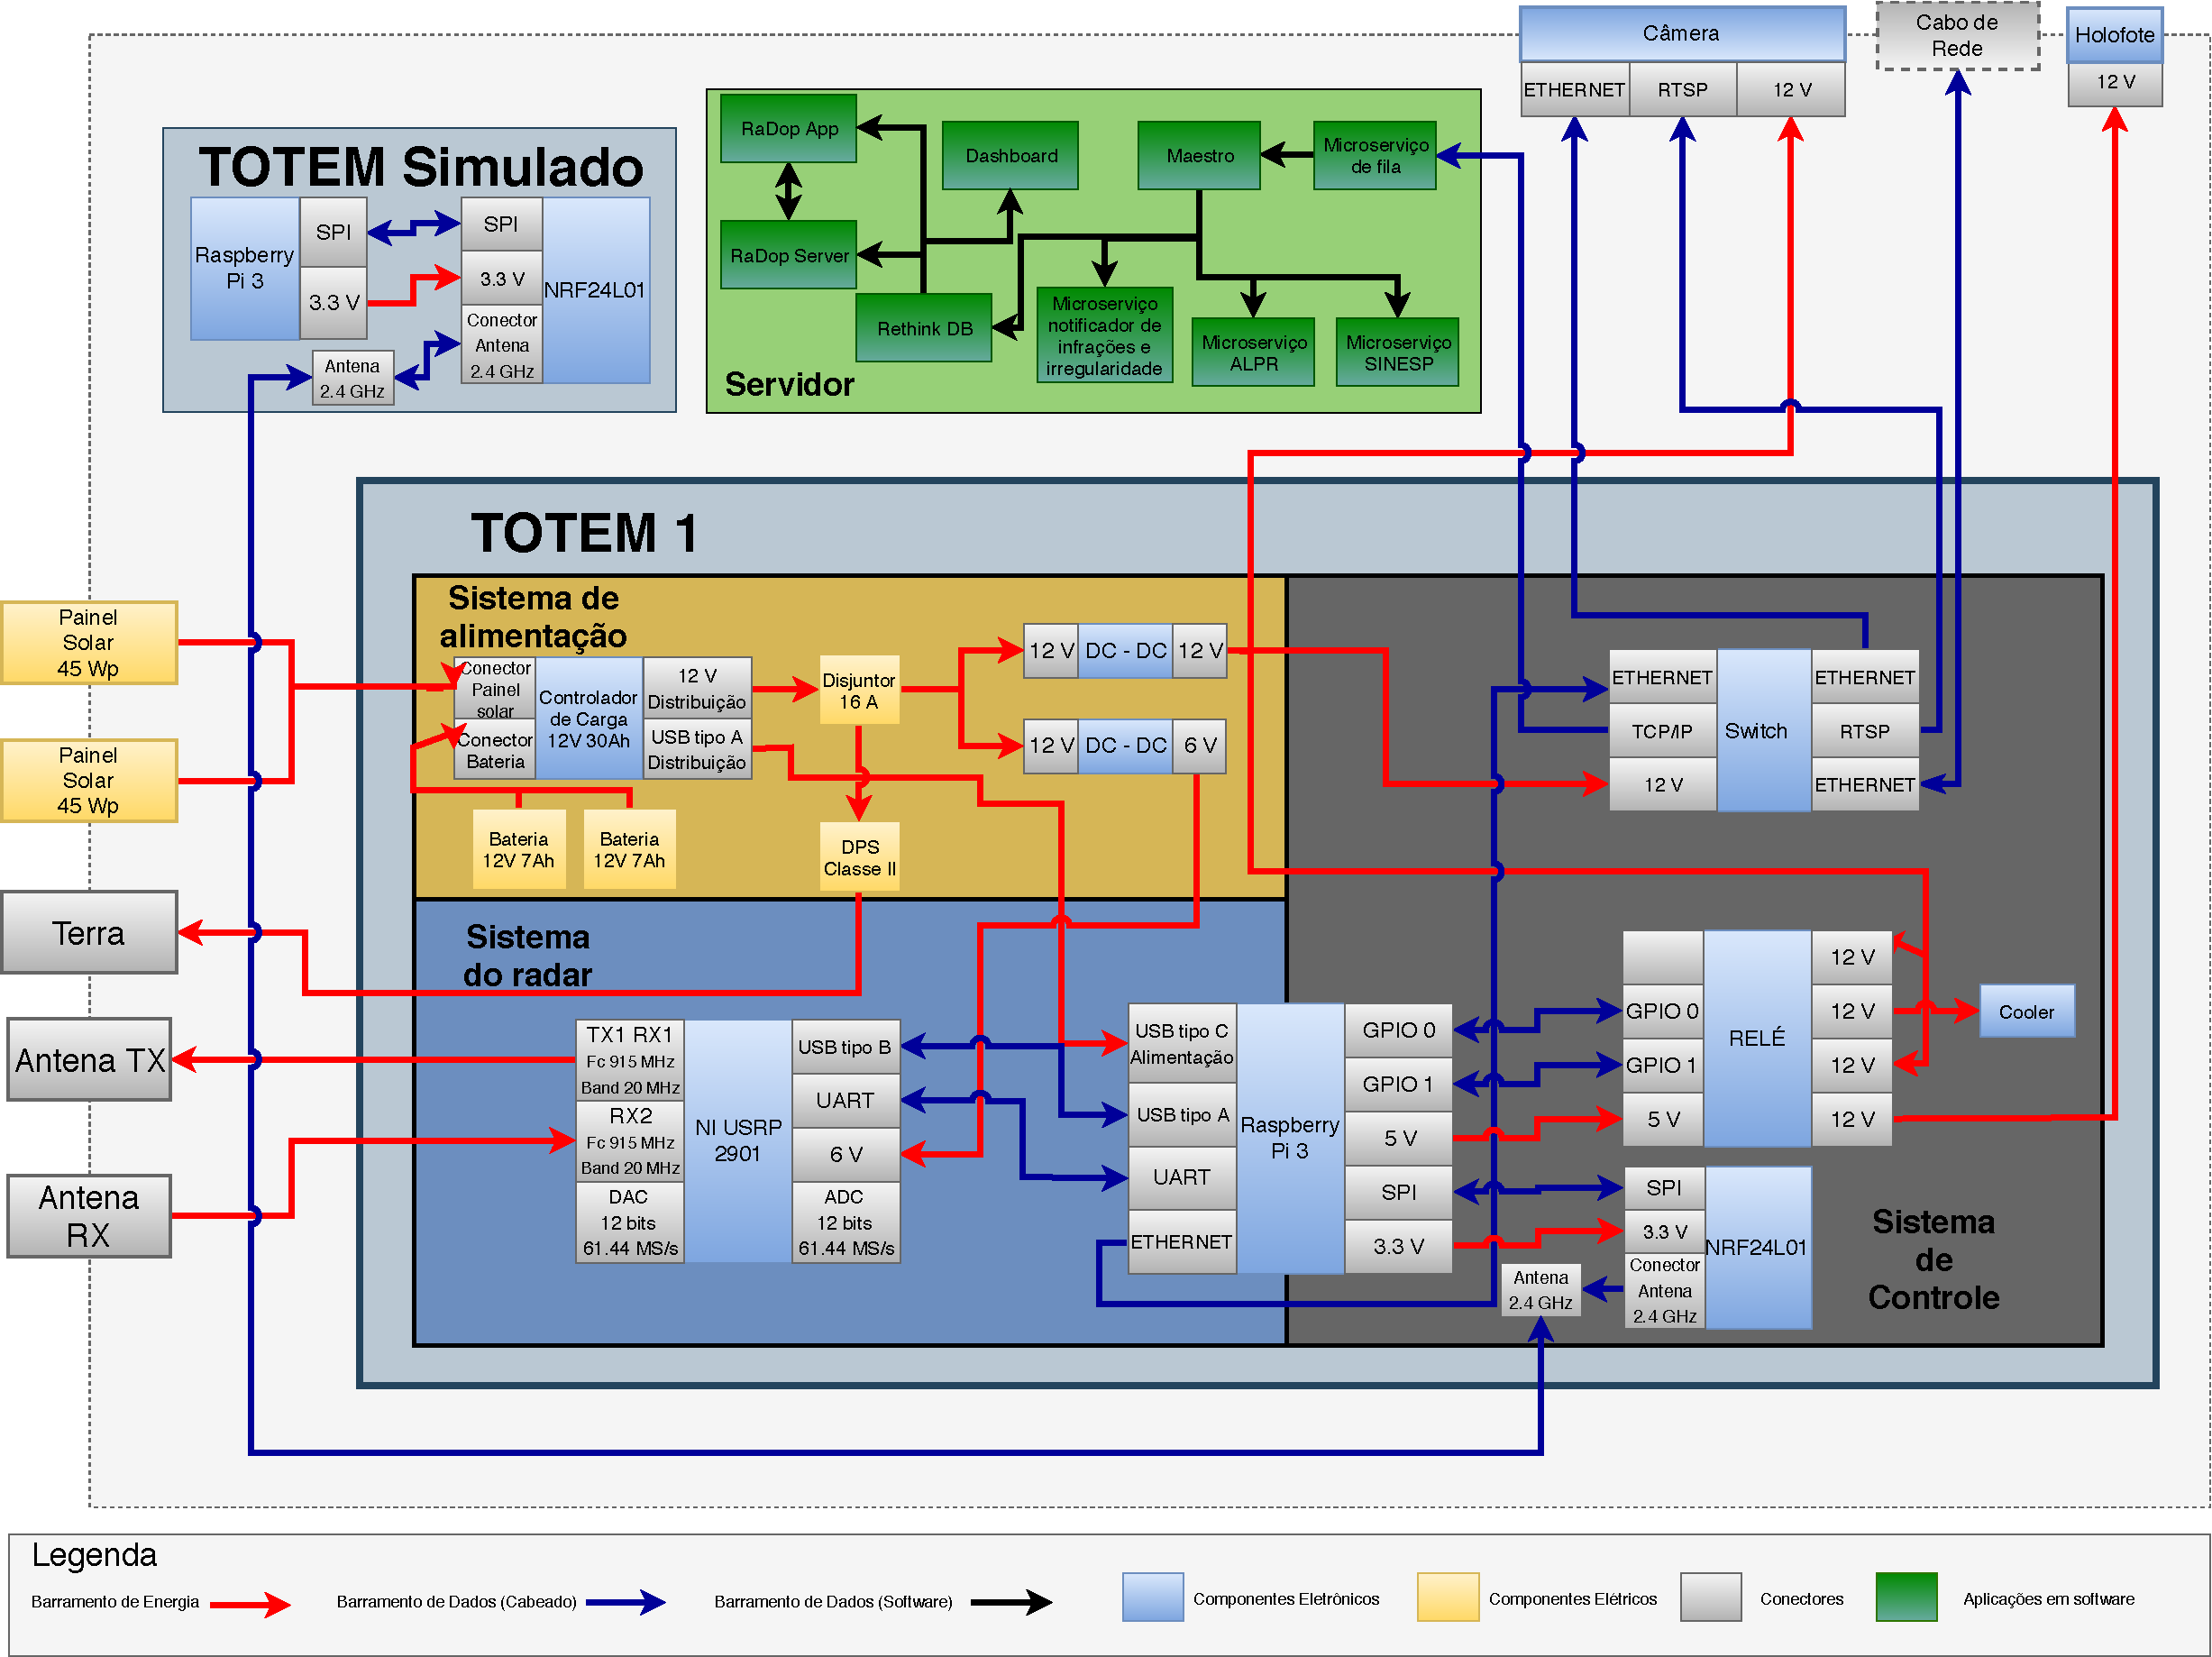
\includegraphics[scale=0.32]{Integracao-3.pdf}
    \caption{Diagrama de integração.}
    \label{fig:planejamento_integracao}
\end{figure}

A integração realizada para o radar foi dividida em pacotes, com o sistema de alimentação, o sistema de radar, o sistema de controle -- que se comunica com o totem simulado e o totem físico -- e o servidor que recebe os dados gerados, vindos do sistema de controle.

\section{Eletrônica-Estrutura-Energia}

A Figura \ref{fig:estrutura} apresenta a estrutura completa com todos os subsistemas físicos presentes no sistema de radar.

\begin{figure}[H]
    \centering
    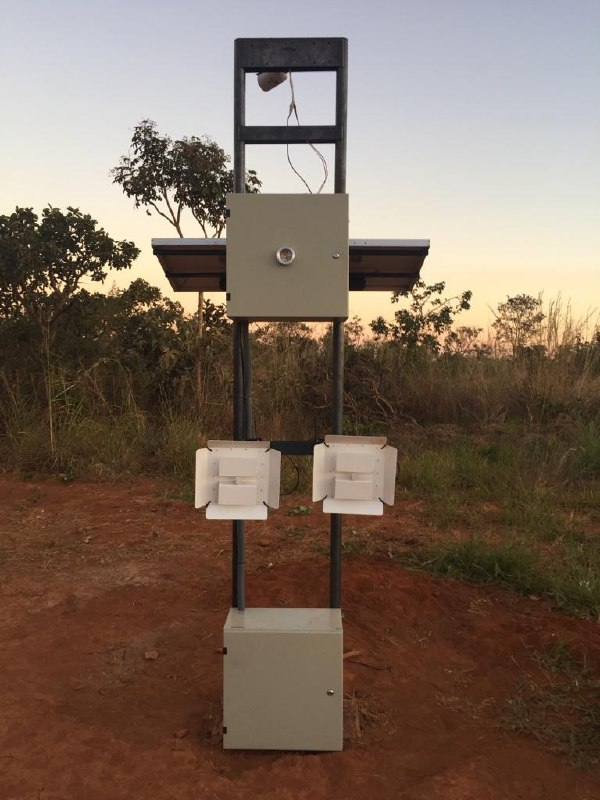
\includegraphics[scale=0.4]{estrutura_toda.jpg}
    \caption{Sistema de radar com a estrutura completa.}
    \label{fig:estrutura}
\end{figure}

Os painéis solares foram instalados no suporte com uma angulação de 15$^{\circ}$, como mostra a Figura \ref{fig:vista}.

\begin{figure}[H]
    \centering
    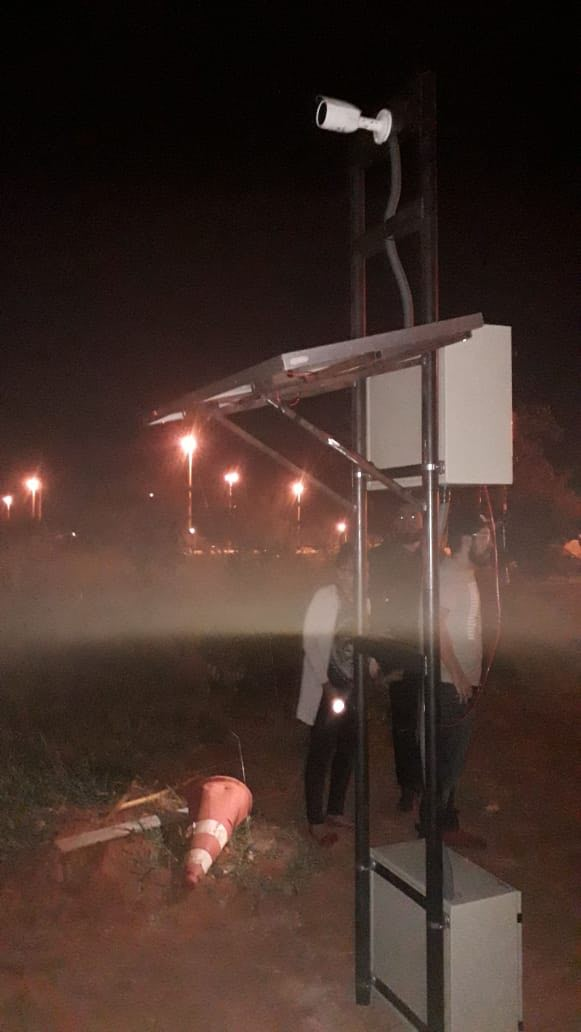
\includegraphics[scale=0.3]{vista_lateral.jpg}
    \caption{Vista lateral do sistema de radar.}
    \label{fig:vista}
\end{figure}

Os painéis estão posicionados atrás da caixa de controle, onde estão dispostos todos os componentes eletrônicos do radar, como mostra a Figura \ref{fig:painel}. A caixa inferior estão dispostas as baterias que alimentam o sistema.
\begin{figure}[H]
    \centering
    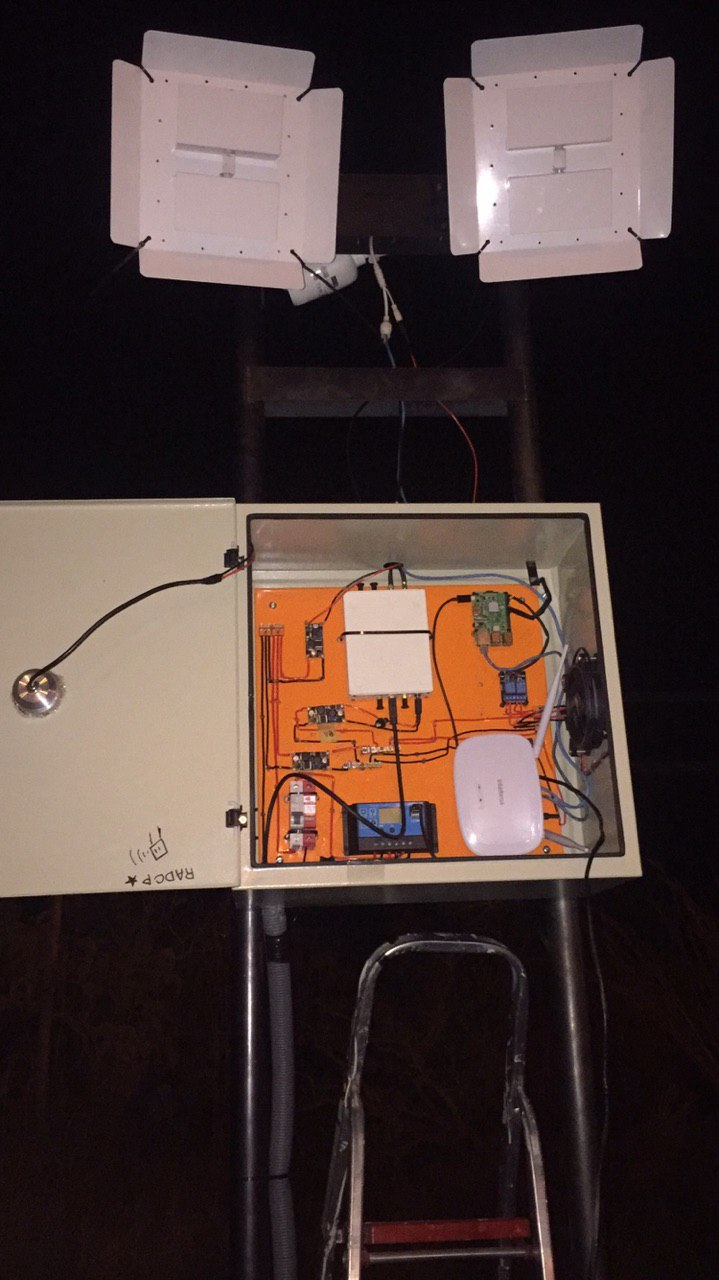
\includegraphics[scale=0.3]{painel_antenas.jpg}
    \caption{Painel de Controle disposto na caixa superior.}
    \label{fig:painel}
\end{figure}

A câmera foi instalada a 3 metros de altura na parte de trás da estrutura, como visto na Figura \ref{fig:vista}, pois a captura feita é da placa traseira do veículo, pelo fato de alguns destes veículos não possuírem placa frontal. Além disso a altura se deve pelo ângulo de ataque da câmera com um melhor posicionamento para uma posterior identificação da placa. Para sua alimentação de 12 V e 0.7 A, seu cabo foi conectado em um barramento de energia controlado por um conversor DC-DC \emph{step up}, que mantém a tensão de saída em 12V.  O testes feitos pela câmera com o veículo resultaram nas Figuras \ref{car1} e \ref{car2}.

\begin{figure}[H]
     \centering
     
     \begin{subfigure}{0.6\textwidth}
         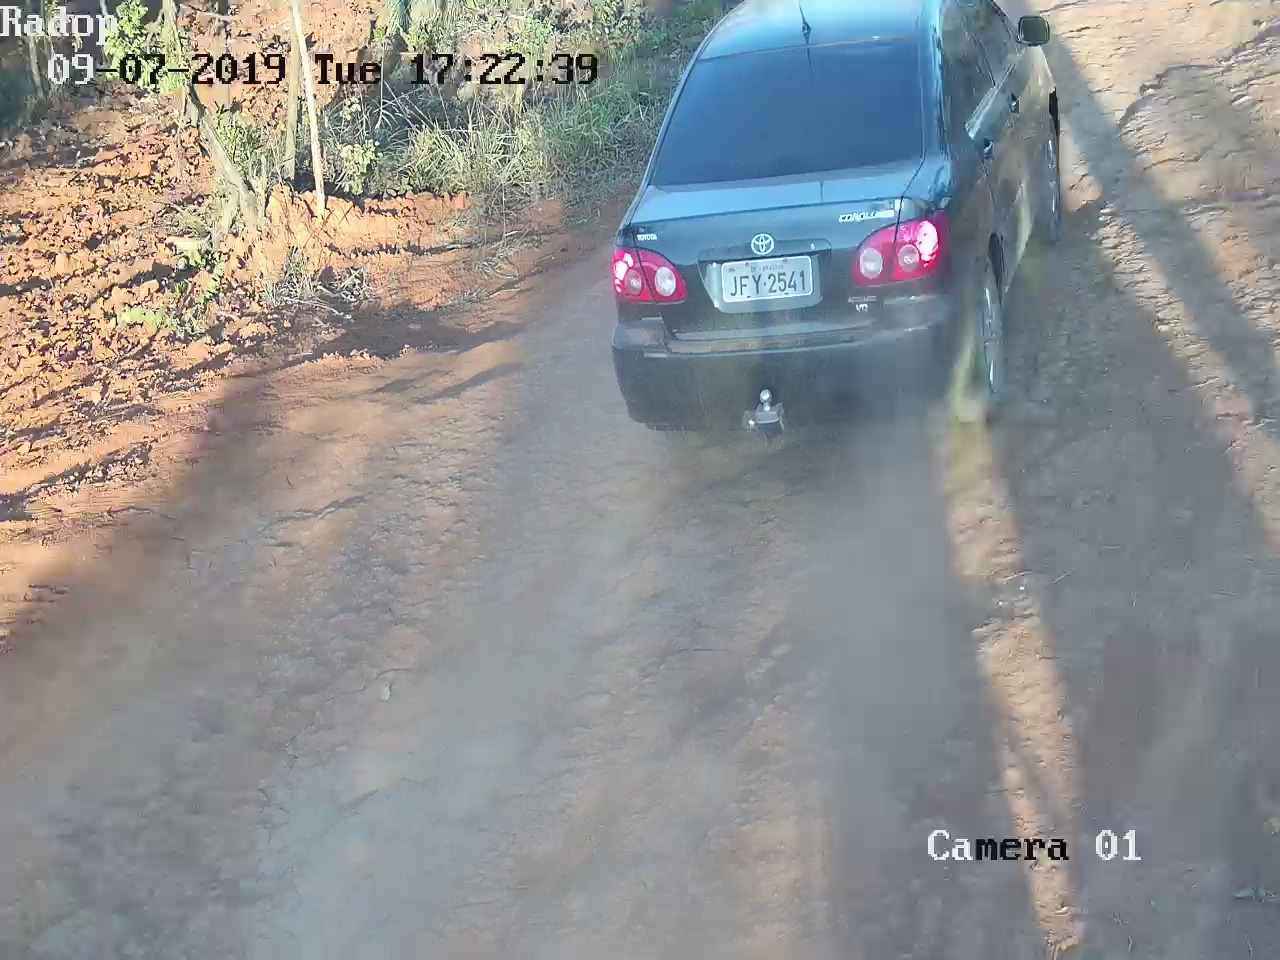
\includegraphics[width=\textwidth]{17_22_44_494390.jpg}
         \caption{Captura feita pela câmera em caso de infração com o carro a uma distância maior.}
         \label{car1}
     \end{subfigure}

     \begin{subfigure}{0.6\textwidth}
         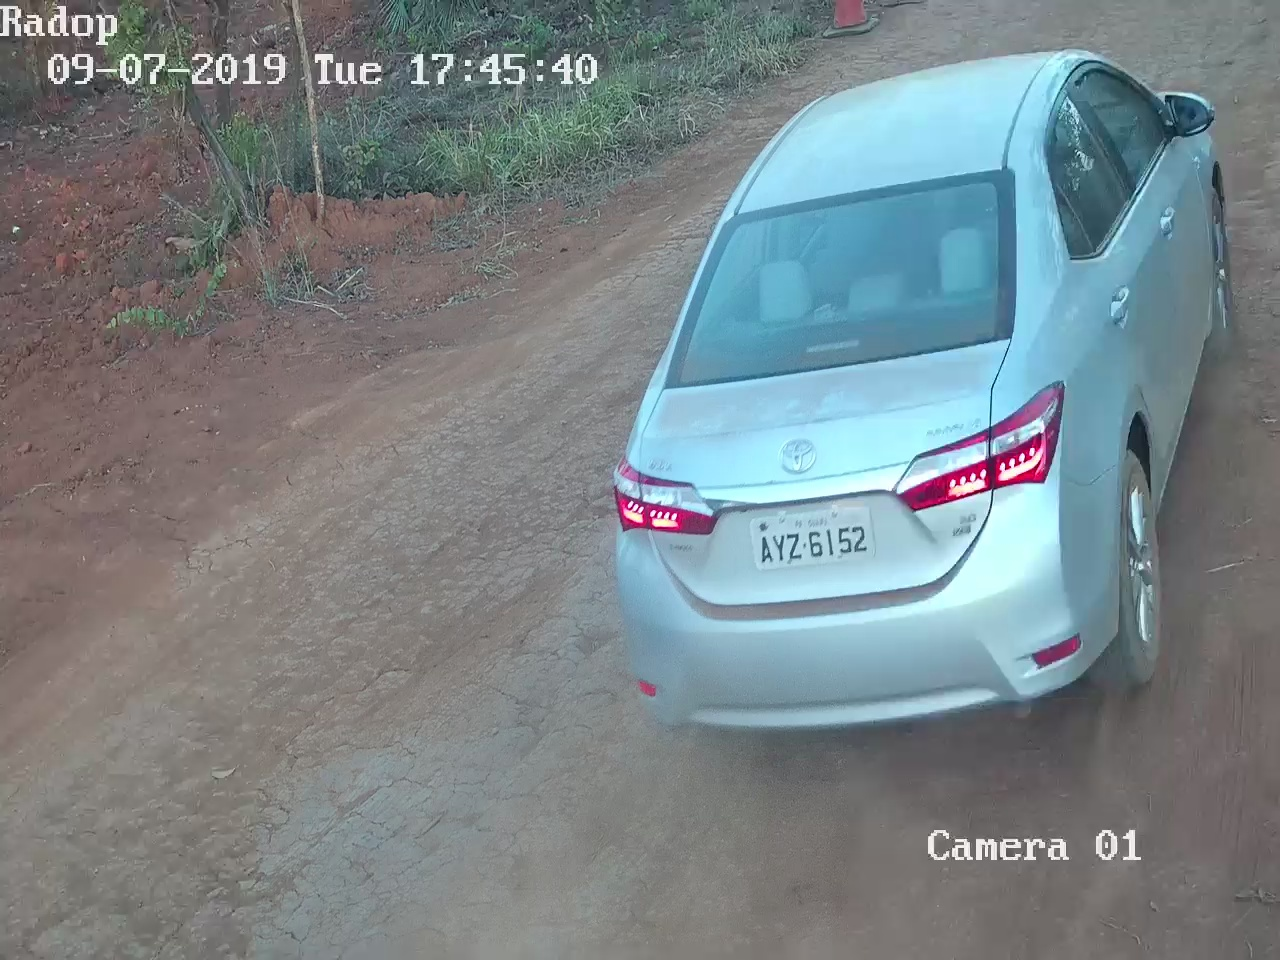
\includegraphics[width=\textwidth]{17_45_44_586283.jpg}
          \caption{Captura feita pela câmera em caso de infração com o carro no centro da área de captura.}
         \label{car2}
     \end{subfigure}
\end{figure}

As antenas foram acopladas em suportes articulados na estrutura, de modo a facilitar o apontamento das antenas.

A Figura \ref{fig:painel_controle} apresenta somente o painel de controle, onde apresenta o controlador de carga que distribui a energia para os componentes eletrônicos e um dispositivo contra surtos para proteção dos mesmos.

\begin{figure}[H]
    \centering
    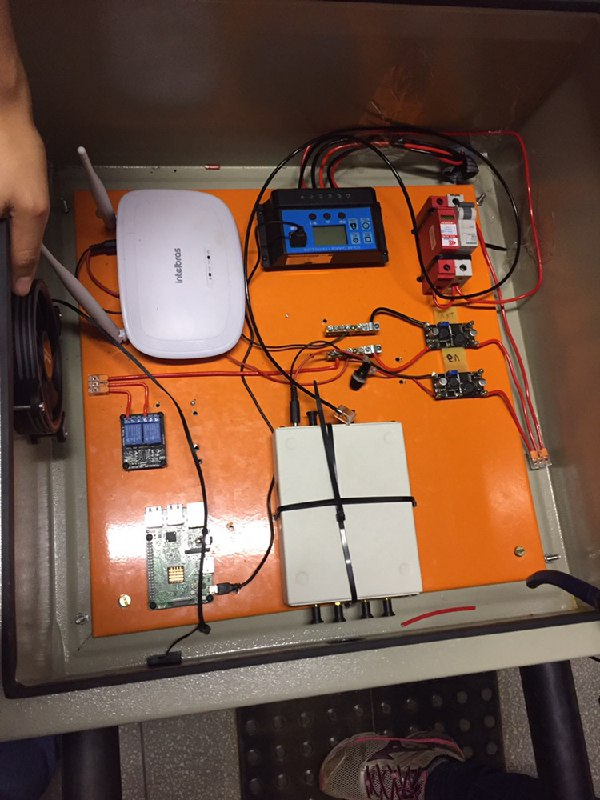
\includegraphics[scale=0.4]{painel_fios.jpg}
    \caption{Painel de controle.}
    \label{fig:painel_controle}
\end{figure}


\section{Eletrônica - Software}

O protocolo que faz comunicação entre a \emph{Raspberry Pi 3} e o servidor é o \emph{Advanced Message Queuing Protocol} (AMQP). O servidor recebe alguns dados do veículo que estiverem transitando acima do limite estabelecido na via. 

Foi definido que os dados enviados no caso de uma infração são: 

    \begin{itemize}
        \item ID do radar: Identificação única do equipamento utilizado, mediante numeração estabelecida pela instituição responsável por administrar os radares e os dados gerados por eles. Este dado é um número inteiro positivo;
        \item Velocidade regulamentada: Velocidade limite para  local da via, conforme determinado pelas normas do CONTRAN \cite{contranVI}. Este dado é um número inteiro positivo;
        \item Velocidade medida: Velocidade  do veículo calculada pelo equipamento. Este dado é um número inteiro;
        \item Velocidade considerada: Velocidade medida subtraída pelo erro máximo admitido previsto na legislação metrológica. Este dado é um número inteiro;
        \item Infração: Natureza da infração cometida. Estes dados são do tipo inteiro, enviados por enumeração. 0, 1 e 2 correspondem, respectivamente, à infração média, grave e gravíssima;
        \item Imagens: As imagens tanto em escala de cinza do carro quanto a imagem pré processada para reconhecimento da placa são codificadas em base64 antes de serem enviadas ao servidor;
        \end{itemize}
        
No caso de envio de dados sobre o funcionamento do radar, os dados enviados são:
    \begin{itemize}
        \item ID do radar: Identificação única do equipamento utilizado, mediante numeração estabelecida pela instituição responsável por administrar os radares e os dados gerados por eles. Este dado é um número inteiro positivo;
        \item Câmera: Retorna se a câmera está ou não funcionando corretamente. Este dado será do tipo \emph{boolean}, sendo verdadeiro para correto funcionamento e falso caso esteja ocorrendo algum problema com esse componente. 
        \item \emph{Raspberry}: Retorna se o NRF24L01 está ou não funcionando corretamente. Este dado será do tipo \emph{boolean}, sendo verdadeiro para correto funcionamento e falso caso esteja ocorrendo algum problema com esse componente.
        \item USRP: Retorna se o USRP está ou não funcionando corretamente.  Este dado será do tipo \emph{boolean}, sendo verdadeiro para correto funcionamento e falso caso esteja ocorrendo algum problema com esse componente.
        \item Funcionamento do radar: Retorna se o radar em geral está funcionando corretamente. Este dado será do tipo \emph{boolean}, sendo verdadeiro para correto funcionamento e falso caso esteja ocorrendo algum problema com esse componente.
        \end{itemize}
    \section{Conclusão}
    
    Nesse projeto foi proposto o desenvolvimento de um sistema de radar de efeito \emph{Doppler} para prevenção de acidentes. Devido as limitações do equipamento utilizado, não foi possível detectar um carro a uma distância considerável, já que a USRP transmitia até 20 dBm, com o amplificador de potência foi alcançado uma potência de 30 dBm, o que melhorou o funcionamento do radar, seria necessário um equipamento que conseguisse mandar uma potência maior para que podesse detectar o carro a distância prevista inicialmente.
    
    O sistema de controle conseguiu um capturar a placa do carro e detectar as bordas da placa, não foi possível concluir com o recorte completo. O sistema sinalizou corretamente e também enviar os dados para o servidor. 
    
    A integração do subsistema de eletrônica não foi realizado devido as dificuldades de embarcar o GNU-RADIO na raspberry, com isso o sistema funcionou de forma separada o sistema do radar e o sistema do controle.
    
    O sistema energético conseguiu alimentar os componentes eletrônicos. Os paínéis solares tiveram uma perda na eficiência devido a inclinação da estrutura que afetou na inclinação dos painéis.
    
    O sistema de estrutura por motivos de burocracia, teve problemas com a fundação, mudando a posição ideal do painel, porém todo o sistema foi concluído e estava funcional.

    
